\documentclass[tikz,border=8pt]{standalone}
\usepackage{amsmath,amssymb}
\usetikzlibrary{arrows.meta,calc,decorations.markings,decorations.pathmorphing,patterns,shapes.geometric,positioning}

\begin{document}
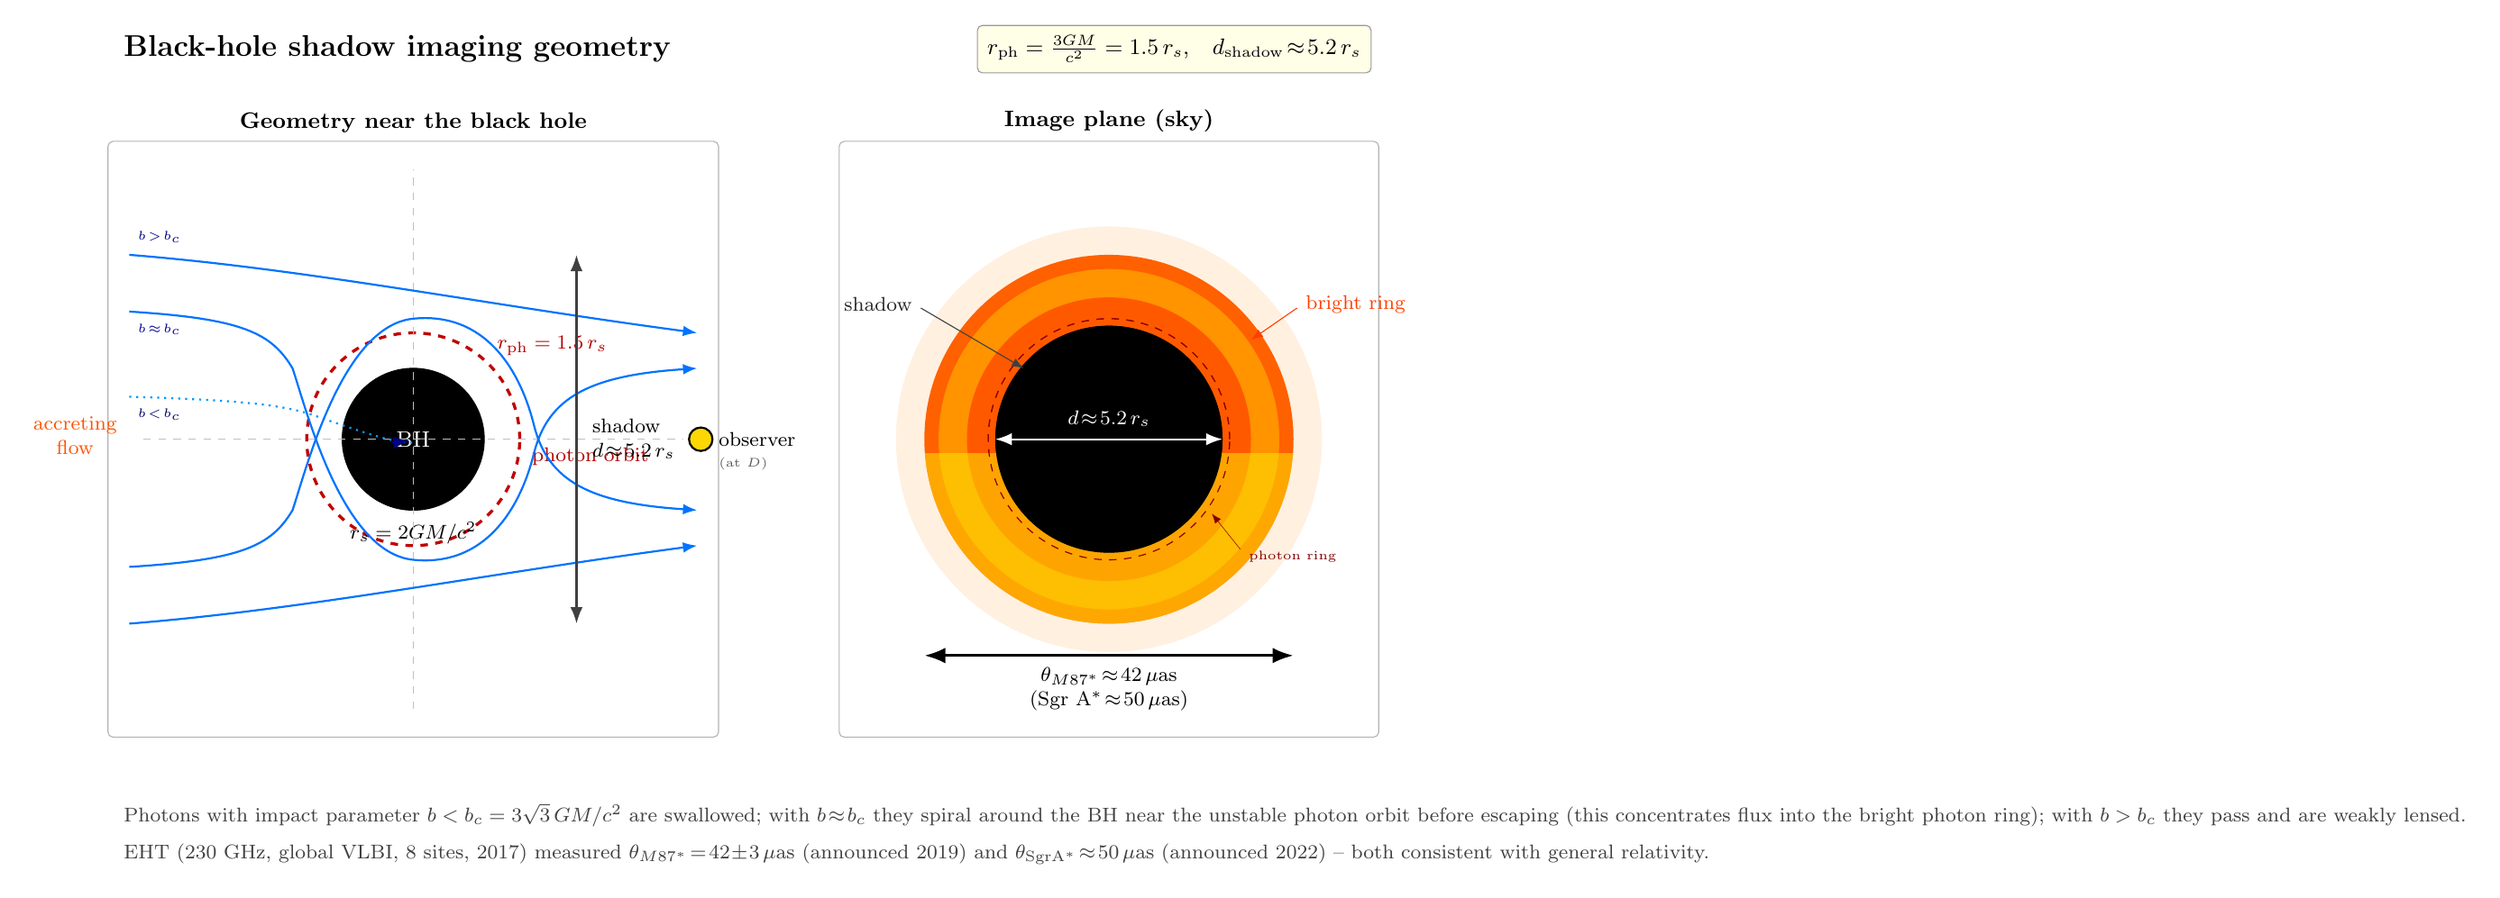
\begin{tikzpicture}[>=Latex,
  bhcore/.style={fill=black, draw=black},
  photonsphere/.style={draw=red!75!black, very thick, dashed},
  raylight/.style={draw=blue!55!cyan, thick, -{Latex[length=2mm]}},
  rayswallow/.style={draw=blue!40!cyan, thick, dotted},
  obs/.style={draw=black, thick, fill=yellow!75!orange},
  brightring/.style={draw=orange!75!red, very thick, fill=orange!50!yellow},
  shadowfill/.style={fill=black},
  framebox/.style={draw=black!30, thin, rounded corners=2pt}]

  % --- Title ---------------------------------------------------------------
  \node[font=\large\bfseries, anchor=west] at (-9.0, 5.5)
    {Black-hole shadow imaging geometry};
  \node[font=\small, draw=black!40, rounded corners=2pt, fill=yellow!10, inner sep=4pt, anchor=east]
    at (8.7, 5.5)
    {$r_{\rm ph}=\tfrac{3GM}{c^{2}}=1.5\,r_{s}$,\quad
     $d_{\rm shadow}\!\approx\!5.2\,r_{s}$};

  % =========================================================================
  % LEFT PANEL: ray-tracing geometry around BH
  % =========================================================================
  \begin{scope}[shift={(-4.8, 0)}]
    \draw[framebox] (-4.3, -4.2) rectangle (4.3, 4.2);
    \node[font=\small\bfseries, anchor=south] at (0, 4.2)
      {Geometry near the black hole};

    % Photon sphere (radius 1.5 in scene units, r_s = 1.0)
    \draw[photonsphere] (0,0) circle (1.5);
    \node[font=\footnotesize, text=red!70!black, anchor=south west]
      at (1.06, 1.06) {$r_{\rm ph}=1.5\,r_{s}$};
    \node[font=\footnotesize, text=red!70!black, anchor=west]
      at (1.55, -0.25) {photon orbit};

    % Event horizon (r_s = 1.0) -- BH black disk
    \fill[bhcore] (0,0) circle (1.0);
    \node[font=\small, text=white, anchor=center] at (0,0) {BH};
    \node[font=\footnotesize, anchor=north, text=black]
      at (0, -1.05) {$r_{s}=2GM/c^{2}$};

    % Coordinate cross (faint)
    \draw[black!25, thin, dashed] (-3.8, 0) -- (3.8, 0);
    \draw[black!25, thin, dashed] (0, -3.8) -- (0, 3.8);

    % --- Rays incoming from the right (observer side) ---
    % Ray A: large b -> deflects mildly, escapes back to right (we follow time-reverse:
    %                   light from the bright accretion flow on left, lensed past BH to observer on right)
    % We draw rays going LEFT-TO-RIGHT (incoming from far left, exiting to far right)
    % to match the bright source on the LEFT of the panel and observer on RIGHT.

    % Ray 1: high b above, only mild bend, escapes to right
    \draw[raylight]
      (-4.0, 2.6) .. controls (-1.5, 2.4) and (1.0, 1.9) .. (4.0, 1.5);
    \node[font=\tiny, text=blue!50!black, anchor=west] at (-4.0, 2.85) {$b\!>\!b_{c}$};

    % Ray 2: critical b ~ b_c, spirals once around BH, escapes
    \draw[raylight, thick]
      (-4.0, 1.8)
      .. controls (-2.4, 1.7) and (-2.0, 1.5) .. (-1.7, 1.0)
      .. controls (-1.5, 0.4) and (-1.0, -1.6) .. (0.0, -1.7)
      .. controls (1.0, -1.8) and (1.5, -1.0) .. (1.7, -0.2)
      .. controls (1.9, 0.6) and (2.5, 0.9) .. (4.0, 1.0);
    \node[font=\tiny, text=blue!60!black, anchor=west] at (-4.0, 1.55)
      {$b\!\approx\!b_{c}$};

    % Ray 3: b < b_c, captured -- spirals into horizon
    \draw[rayswallow, thick]
      (-4.0, 0.6)
      .. controls (-2.5, 0.55) and (-1.8, 0.5) .. (-1.3, 0.3)
      .. controls (-0.7, 0.1) and (-0.3, -0.05) .. (0.0, -0.05);
    \node[font=\tiny, text=blue!40!black, anchor=west] at (-4.0, 0.35)
      {$b\!<\!b_{c}$};
    % swallow arrow showing capture into BH
    \draw[->, thick, blue!50!black, dotted] (-0.3, -0.05) -- (-0.05, -0.02);

    % Ray 4 (mirror low side): b ~ b_c on negative-y side, escapes
    \draw[raylight, thick]
      (-4.0, -1.8)
      .. controls (-2.4, -1.7) and (-2.0, -1.5) .. (-1.7, -1.0)
      .. controls (-1.5, -0.4) and (-1.0, 1.6) .. (0.0, 1.7)
      .. controls (1.0, 1.8) and (1.5, 1.0) .. (1.7, 0.2)
      .. controls (1.9, -0.6) and (2.5, -0.9) .. (4.0, -1.0);

    % Ray 5: high b below, only mild bend
    \draw[raylight]
      (-4.0, -2.6) .. controls (-1.5, -2.4) and (1.0, -1.9) .. (4.0, -1.5);

    % Distant source label (far left)
    \node[font=\footnotesize, anchor=east, align=center, text=orange!65!red]
      at (-4.05, 0.05) {accreting\\ flow};

    % Observer (far right)
    \node[obs, circle, minimum size=8pt] (Obs) at (4.05, 0) {};
    \node[font=\footnotesize, anchor=west] at (4.18, 0) {observer};
    \node[font=\tiny, anchor=west, text=black!65] at (4.18, -0.35) {(at $D$)};

    % shadow diameter callout (vertical bar near horizon)
    \draw[<->, thick, black!75]
      (2.3, -2.6) -- (2.3, 2.6);
    \node[font=\footnotesize, anchor=west, align=left]
      at (2.4, 0)
      {shadow\\ $d\!\approx\!5.2\,r_{s}$};

  \end{scope}

  % =========================================================================
  % RIGHT PANEL: image-plane (sky) reconstruction -- M87*-style ring
  % =========================================================================
  \begin{scope}[shift={(5.0, 0)}]
    \draw[framebox] (-3.8, -4.2) rectangle (3.8, 4.2);
    \node[font=\small\bfseries, anchor=south] at (0, 4.2)
      {Image plane (sky)};

    % Outer faint glow (background)
    \fill[orange!12!white] (0,0) circle (3.0);

    % Bright ring: annulus orange-red
    \fill[orange!75!red] (0,0) circle (2.6);
    \fill[orange!85!yellow] (0,0) circle (2.4);
    \fill[orange!70!red] (0,0) circle (2.0);
    % central shadow
    \fill[shadowfill] (0,0) circle (1.6);
    % photon ring outline (subtle)
    \draw[red!55!black, thin, dashed] (0,0) circle (1.7);

    % Doppler-bright bottom (asymmetry, like M87*)
    \begin{scope}
      \clip (0,0) circle (2.6);
      \fill[yellow!85!orange, opacity=0.55]
        (-3.0, -3.0) rectangle (3.0, -0.2);
    \end{scope}
    % Re-paint shadow to keep it black
    \fill[shadowfill] (0,0) circle (1.6);
    \draw[red!55!black, thin, dashed] (0,0) circle (1.7);

    % Diameter measurement
    \draw[<->, thick, white]
      (-1.6, 0) -- (1.6, 0);
    \node[font=\footnotesize, text=white, anchor=south] at (0, 0.05)
      {$d\!\approx\!5.2\,r_{s}$};

    % Angular size
    \draw[<->, very thick, black]
      (-2.6, -3.05) -- (2.6, -3.05);
    \node[font=\footnotesize, anchor=north, align=center] at (0, -3.1)
      {$\theta_{M87^{*}}\!\approx\!42\,\mu\mathrm{as}$\\
       (Sgr A$^{*}\!\approx\!50\,\mu\mathrm{as}$)};

    % Label: bright ring
    \node[font=\footnotesize, text=orange!50!red, anchor=west]
      at (2.65, 1.9) {bright ring};
    \draw[->, thin, orange!50!red]
      (2.65, 1.85) -- (2.0, 1.4);

    % Label: shadow
    \node[font=\footnotesize, text=black!85, anchor=east]
      at (-2.65, 1.9) {shadow};
    \draw[->, thin, black!75]
      (-2.65, 1.85) -- (-1.2, 1.0);

    % Label: photon ring
    \node[font=\tiny, text=red!50!black, anchor=west]
      at (1.85, -1.65) {photon ring};
    \draw[->, very thin, red!50!black]
      (1.85, -1.55) -- (1.45, -1.05);

  \end{scope}

  % =========================================================================
  % BOTTOM legend / equations
  % =========================================================================
  \node[font=\footnotesize, anchor=west, align=left, text=black!75]
    at (-9.0, -5.3)
    {Photons with impact parameter $b<b_{c}=3\sqrt{3}\,GM/c^{2}$ are swallowed; with
     $b\!\approx\!b_{c}$ they spiral around the BH near the unstable photon orbit
     before escaping (this concentrates flux into the bright photon ring);
     with $b>b_{c}$ they pass and are weakly lensed.};
  \node[font=\footnotesize, anchor=west, align=left, text=black!75]
    at (-9.0, -5.85)
    {EHT (230 GHz, global VLBI, 8 sites, 2017) measured $\theta_{M87^{*}}\!=\!42\!\pm\!3\,\mu\mathrm{as}$
     (announced 2019) and $\theta_{\rm Sgr A^{*}}\!\approx\!50\,\mu\mathrm{as}$ (announced 2022)
     -- both consistent with general relativity.};

\end{tikzpicture}
\end{document}
